In 1915 Albert Einstein published the theory of general relativity which describes gravity as the curvature of four-dimensional spacetime. General relativity predicts the existence of gravitational radiation. Gravitational waves travel at the speed of light, carrying energy and information about the sources that generate them. Sources of gravitational waves include: core collapse supernova, compact-object binary inspirals, the gravitational-wave stochastic background, and isolated neutron stars. In this thesis we will focus on gravitational waves from binary neutron stars. As the neutron stars orbit around each other, they lose energy due to gravitational-wave emission causing their orbit to shrink and the neutron stars to merge. The Hulse-Taylor binary~\cite{Hulse:1974eb} indirectly confirmed the existence of gravitational waves. In 1988, Driever, Weiss, and Thorne proposed the construction of the Laser Interferometer Gravitational-wave Observatort (LIGO), a ground-based interferometer to directly detect gravitational waves, test Einstein's theory, and study the properties of gravitational-wave sources. The first-generation LIGO~\cite{Barish:1999} detectors began searching for gravitational waves in 2002. The second-generation Advanced LIGO~\cite{TheLIGOScientific:2014jea} and Advanced Virgo~\cite{TheVirgo:2014hva} detectors made the first direct detection of gravitational waves in 2015, the first detection of a binary neutron star merger in 2017, and to date have completed three observing runs and detected fifty gravitational wave signals from the merger of compact-object binaries. Planning is underway for the construction of a third-generation U.S.~gravitational-wave observatory known as Cosmic Explorer; this detector will have an order of magnitude better sensitivity that Advanced LIGO and will see binary black holes to the edge of the visible universe.

Advanced LIGO detected the first gravitational wave signal from a binary black hole merger, GW150914~\cite{Abbott:2016blz}, during its first observing run. Two more binary black hole mergers were detected soon after in the same observing run~\cite{TheLIGOScientific:2016pea, Nitz:2018imz}. The first binary neutron star inspiral, GW170817~\cite{TheLIGOScientific:2017qsa}, was detected during the second observing run. In addition to the gravitational-wave detection, the merger was observed across the full electromagnetic spectrum~\cite{GBM:2017lvd}, making it the first multi-messenger gravitational-wave detection and contributed to answering outstanding questions in physics such as the origin of short gamma-ray bursts, the nature of kilonovae, and the creation of the r-process elements. Seven binary black hole detections were also made in the second observing run on top of the binary neutron star detection~\cite{Abbott:2017gyy,Abbott:2017oio,Abbott:2017vtc,LIGOScientific:2018mvr}. In the third observing run 39 additional detections were confirmed~\cite{Abbott:2020niy} with one binary neutron star merger~\cite{Abbott:2020uma}, 36 binary black hole mergers~\cite{Abbott:2020niy,Abbott:2020tfl,LIGOScientific:2020stg}, and the first black hole compact object merger, where the compact object could be a highest mass neutron star or a lowest mass black hole ever discovered~\cite{Abbott:2020khf}. With the gravitational-wave detections being made by Advanced LIGO and Virgo becoming regular, we have the ability to answer exciting questions about binary physics and the formation of these compact object binaries. In this thesis we study the detection and measurement of eccentric binary neutron stars and the use of eccentricity to make inferences the formation channel of the binary.

\section{Eccentricity}

The Hulse-Taylor binary was discovered in 1974~\cite{Hulse:1974eb} and is composed of a neutron star and a pulsar with an eccentricity of $e=0.615$ and a period of $7.75$~hours. It was the first binary pulsar discovered and led to a Nobel prize for Hulse and Taylor~\cite{Buehrke:1993nd}. As a binary emits gravitational waves orbital energy is lost which causes a decrease in the binary's orbital period~\cite{Peters:1963ux, Peters:1964zz}. After thirty years of observations the decay in orbital period of the Hulse-Taylor binary was measured and found to be consistent with the emission of gravitational waves~\cite{Weisberg:2004hi}. Sixteen additional double neutron star systems have been observed through radio surveys of the Milky Way field \cite{Martinez:2017jbp,Tauris:2017omb,Cameron:2017ody,Stovall:2018ouw,Lynch:2018zxo} with eccentricities varying from $0.06$ to $0.828$ \cite{Zhu:2017znf,Andrews:2019vou}. As the orbit of a binary neutron star evolves, the orbital eccentricity of the binary will decrease~\cite{Peters:1964zz}. Eccentricity is radiated away very efficiently causing the binary to circularize. Given the significant time to merger of the binary like the Hulse-Taylor pulsar, by the time that the gravitational waves enter the LIGO-Virgo band, the binary's orbit will have circularized. However, formation channels have been proposed in which binaries may still have residual eccentricity when they enter the LIGO-Virgo band.

Eccentricity describes how much an object's orbit deviates from a circle as seen in Fig.~\ref{fig:eccentricity}. The shape and motion of an object in an elliptical orbit can be described by Kepler's first law
\begin{equation}
    r(\theta) = \frac{a(1-e^2)}{1-e\cos(\theta)},
\end{equation}
where $r(\theta)$ is the position of a particle in the orbit assuming the origin is at one foci of the ellipse, $a$ is the semimajor axis, $e$ is the eccentricity, and $\theta$ is the true anomaly. The true anomaly is an angular parameter that defines the position of a particle moving along a Keplerian orbit. The angle defined is the angle between the closest point to the body that is being orbited and the current position of the particle in its orbit. 

In the Newtonian description of gravity, a stars have closed orbits around their center of mass with the motion described by Kepler's laws. This Newtonian description is valid in the slow motion and weak gravitational-field limit. For example, it does not accurately describe the perihelion precession of Mercury. Einstein's theory of general relativity, however, accurately predicts the precession of Mercury and also predicts the orbital decay of a binary as it radiates gravitational waves.

As compact objects orbit around each other they emit gravitational waves. Binaries without eccentricity evolve in a sequence of circular orbits where the frequency and amplitude are monotonically increasing as the stars inspiral together. However, binaries with eccentricity have weaker gravitational wave emission when the compact objects are far apart and a stronger emission when the compact objects are close. This emission of gravitational waves in binaries with eccentricity will cause the orbit of the binary to become smaller and more circular. In most cases as gravitational waves are emitted the binary the binary loses energy and angular momentum. In the case of eccentric binaries, the semi-major axis and eccentricity also decay over time. The orbital decay for an eccentric binary system is described in Sec.~\ref{GW-eccentricity} and in Refs.~\cite{Peters:1963ux,Peters:1964zz}.

Gravitational waves can be detected in searches with ground based detectors. For systems that have circularized eccentricity can be neglected. However, this means that binaries with residual eccentricity may be missed. Even though a binary system may be detected by a search that neglects eccentricity, the system may have residual eccentricity that can be measured. Parameter estimation can be used to measure or place an upper limit on the eccentricity of the binary. The Hulse-Taylor binary had a significant amount of eccentricity $e=0.615$ and a short orbital period~\cite{Hulse:1974eb} during its discovery. As a results of the high eccentricity and short orbital period suggestions about the formation of the binary have been made~\cite{Flannery1975,DeLoore1975}. Depending on the detected or measured eccentricity of the binary we can gain knowledge about the formation of the binary. 

\section{Gravitational-wave Detectors}

Advanced LIGO~\cite{TheLIGOScientific:2014jea} and Advanced Virgo~\cite{TheVirgo:2014hva} are gravitational-wave detectors with 4~km long arms in a worldwide detector network. The Advanced LIGO detectors are located in Hanford, Washington and Livingston, Louisiana, while the Virgo detector is located in Pisa, Italy. These detectors are Michelson interferometers with a Fabry-Perot cavity in each arm to build up the phase introduced by a change in the length of the arms. When a gravitational-wave passes through the detectors, there will be a small change in the light travel time in the arms. The change in the arms is measured as a phase difference over a period of time and from that a gravitational-wave signal can be measured. The lower frequency sensitivity limit on the Advanced LIGO and Virgo detectors are 10~Hz and the detectors are sensitive to sources in the 10-1000~Hz band of the gravitational-wave spectrum. 

The strain sensitivity of the detectors is the strain, $h$, a source must have at a specific frequency to detectable. As a gravitational wave travels away from the binary system it will cause space-time to be stretched and squeezed. A gravitational wave with stain amplitude, $h$, will change the length of the arms $\Delta L$ as it passes through a detector with arms of length, $L$, and can be written as
\begin{equation}\label{eq:strain}
    h \sim \frac{\Delta L}{L}.
\end{equation}
The sensitivity of the detectors or noise floor is determined by environmental, thermal, quantum, and other noise sources~\cite{Martynov:2016fzi}. Environmental noise included seismic motion and acoustic and magnetic noises. The thermal noise is determined by set parameters in the interferometer, such as beam size and material properties. The quantum noise is dependent on the input laser power and the signal recycling mirror transmission. The signal recycling mirror reflects the light back into the detector~\cite{Meers:1988wp}. The next stage of proposed detector upgrades to Advanced LIGO is referred to as A+ which will further increase the sensitivity of the LIGO detectors~\cite{A+}. 

Future gravitational-wave detectors, like Cosmic Explorer~\cite{Reitze:2019iox} and Einstein Telescope~\cite{Punturo:2010zz}, have been proposed. We will focus on Cosmic Explorer in this thesis. Cosmic Explorer is a two-stage ground based gravitational-wave detector with 40~km arms that improves on the Advanced LIGO design. Since the arms of Cosmic Explorer are 10 times as long as that of Advanced LIGO and Advanced Virgo, the detector will be 10 times more sensitivity as shown by Eq.~\ref{eq:strain} In the first stage (CE1) the detector will scale up current Advanced LIGO technology to create a detector with arms that are close to the wavelength of a gravitational-wave signal. The second stage (CE2) upgrades the optics of the detector achieve an order of magnitude sensitivity beyond that of Advanced LIGO~\cite{Reitze:2019dyk}. The low-frequency sensitivity limit of Cosmic Explorer is expected to be a factor of two smaller than that of Advanced LIGO, pushing the limit from 10~Hz to 5~Hz as can be seen in Fig.~\ref{fig:noisecurves}. Cosmic Explorer will also be sensitive to sources in the 5-4000~Hz band of the gravitational-wave spectrum. 

The last stage of detector upgrades, A+, is expected to be able to detect binary neutron star mergers out to a distance of 330~Mpc and Virgo is expected to have a distance of $150-260$~Mpc at design sensitivity~\cite{Aasi:2013wya}. Cosmic Explorer is expected to be able to detect binary neutron star mergers out to a distance of $\sim 2$~Gpc. The addition of another detector to the detector network would significantly improve the ability to determine a location of a detection in the sky.

\section{Formation of Compact Object Binary Sources}

The compact object mergers that Advanced LIGO and Virgo observe are the last stage in the evolution of massive compact object binary systems. Unfortunately the formation of these binaries is difficult to discern. Typically binaries form either in the plane of the galaxy, or field,~\cite{Smarr1976,Canal:1990dz,PortegiesZwart1:1997zn,Belczynski:2018ptv,Vigna-Gomez:2018dza,Giacobbo:2018etu,Mapelli:2018wys,Andrews:2019vou,Kalogera:2006uj,Kowalska:2010qg,Tauris:2017omb,Chruslinska:2017odi}, where two stars that are born together and their evolution is solely dependent on the interactions between the components, or in dynamical environments~\cite{Heggie:1975tg,Grindlay:2005ym,Ivanova:2007bu,Petrovich:2017otm,Sigurdsson:1993zrm,PortegiesZwart:1999nm,Oleary:2008myb,Antonini:2012ad, Rodriguez:2015,Rodriguez:2016,Rodriguez:2016big,Rodriguez:2018pss, Yu:2020iqj}, where the interactions in dense stellar environments are crucial to the evolution of the binary. Most binaries are expected to have formed in the field and will have eccentricity $e \leq 10^{-4}$ by the time they merge~\cite{Peters:1964zz,Hinder:2007qu,Kowalska:2010qg} making them detectable by matched-filter searches that neglect eccentricity \cite{Martel:1999tm,Cokelaer:2009hj,Brown:2009ng,Huerta:2013qb}. However, binaries formed in dynamical environments may retain residual eccentricity $e \geq 0.1$ when they enter the LIGO-Virgo band~\cite{Oleary:2008myb,Heggie:1975tg,Rodriguez:2015,Rodriguez:2016,Rodriguez:2016big,Rodriguez:2018pss,Yu:2020iqj}.   

Binaries in the field typically decrease the separation of their orbit due to the common envelope phase~\cite{Postnov:2006hka} in the evolution of the binary. When a binary undergoes the common envelope phase, the more massive star, primary star, leaves the main sequence phase and rapidly expands. Once the radius crosses the Roche Lobe radius it transfers mass to the less massive star, secondary star, that is still in the main sequence phase. Once mass transfer ends the massive star loses its hydrogen envelope, turns into a helium burning core and eventually goes through a core-collapse supernova explosion to end up a compact object, either a black hole or neutron star. Once the primary star has become a compact object, the secondary star eventually leaves its main sequence phase and the secondary star goes through the same process as the primary. The mass transfer of the secondary star is unstable, which results in the two stars evolving in a shared envelope. This causes the compact object to spiral into the dense stellar environment shrinking the orbit of the binary~\cite{Postnov:2006hka,Ivanova:2012vx}. There are two usual outcomes after the inspiral phase of the binary. The envelope could get ejected due to a deposit of orbital energy which would leave a binary composed of the secondary star and a compact object. Once the secondary star undergoes a supernova explosion it will collapse to a black hole. If the system survives the explosion a close compact object binary is formed which emits gravitational waves in the LIGO-Virgo band and merges within the lifetime of the universe. If the envelope is not ejected, the compact object and companion star could merge and become a single compact object. 

Binaries that form dynamically interact with stars or compact objects in dense stellar environments, like globular clusters or galactic nuclei. One such method is when binaries shrink their orbits and merge due to three or four-body interactions with other stars, typically called gravitational-wave captures. During the three or four-body interactions there is a release of strong gravitational-wave emission that brings the orbit closer to merger. A specific example of a three-body interaction is called an exchange encounter~\cite{Ivanova:2006xp, Ivanova:2007bu}. In an exchange encounter an existing binary will undergo interactions with a third star or compact object. The interactions will cause one of the components in the binary to be thrown out and replaced by third star or object~\cite{Heggie:1996dr}. These binaries may still have significant residual eccentricity when their gravitational waves enter the LIGO-Virgo band. Measurements of the eccentricity of the two binary neutron star mergers, GW170817 and GW190425, were made. Based on the upper limit estimates of their eccentricity the binaries were most likely formed in the field (see Sec.~\ref{ch:bns-pe} for detail).

In Chapter~\ref{ch:eccentric-search}, we describe the results of a search for eccentric binary neutron star mergers. We used matched filtering methods and waveforms that model the gravitational waves from low eccentricity systems to detect potential gravitational-wave signals in the first and second observing runs of Advanced LIGO and Virgo. We use the results of search to place an upper limit on the binary neutron star merger rate and determine how many years of data would be needed to constrain current binary neutron star merger rates. In Chapter~\ref{ch:bns-pe}, we use Bayesian parameter estimation in the PyCBC Inference~\cite{Biwer:2018osg} toolkit to measure parameters of interest of the two binary neutron star mergers from the first and second observing runs. This study concentrated on measuring the eccentricity of the two detections using full parameter estimation and compared that with similar work done for a binary neutron star detection. In Chapter~\ref{ch:3G-eccen-prospects}, we determine Cosmic Explorer's ability to detect and measure the eccentricity of eccentric gravitational-wave signals. We non-eccentric and eccentric template banks as well as simulations of eccentric signals to determine the eccentricity that Cosmic Explorer will be sensitive to in searches and parameter estimation. We also determine the computational cost of a search in Cosmic Explorer compared to previous searches.

\begin{figure}[p]
  \centering
  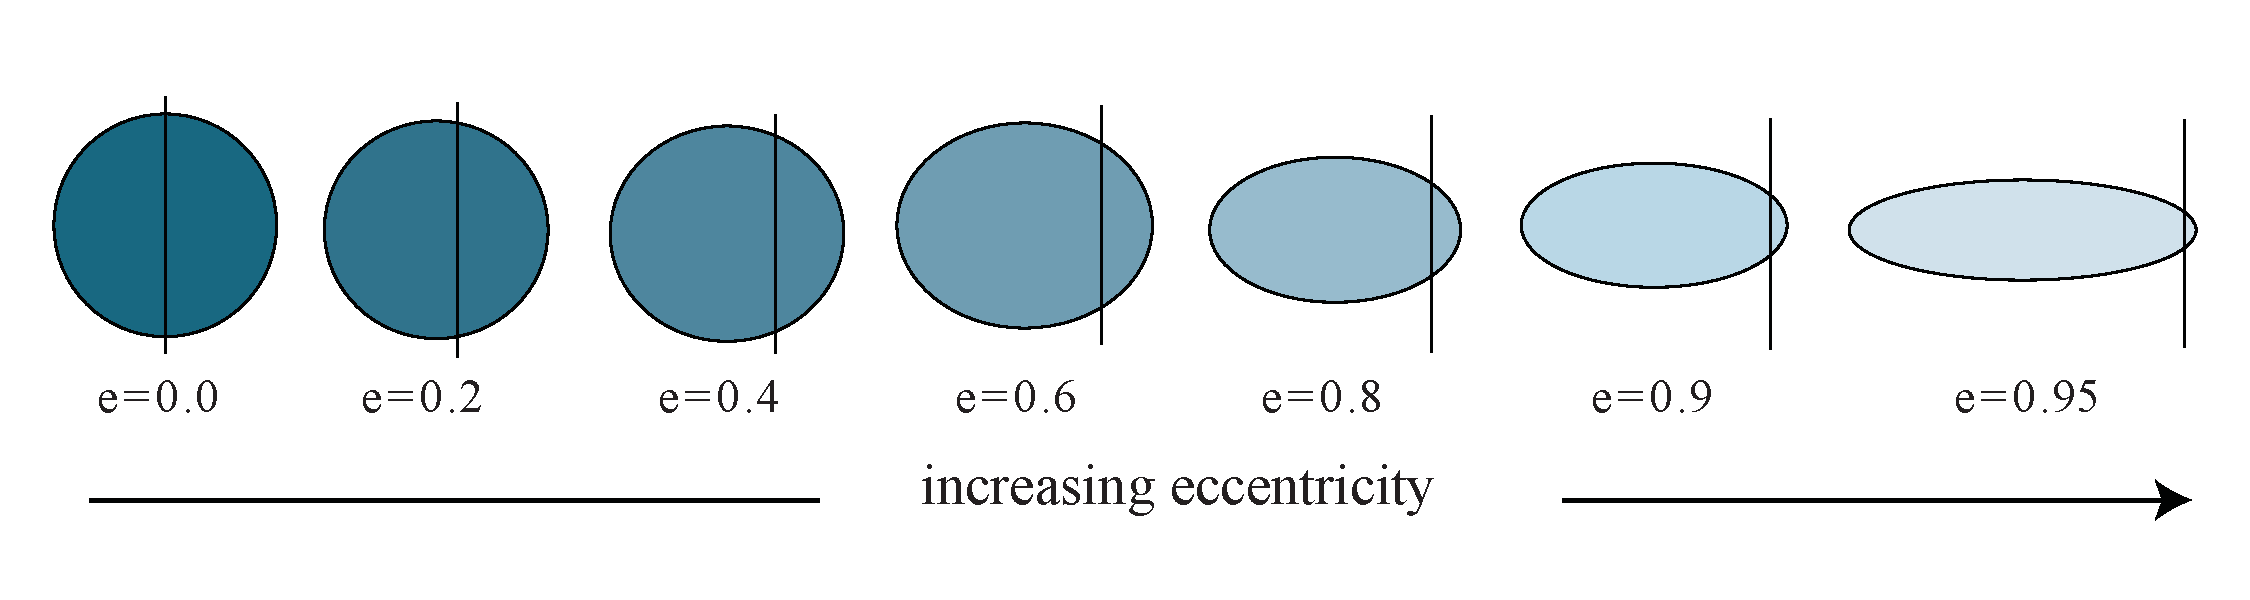
\includegraphics[width=\textwidth]{Figures/Introduction/eccentricity.pdf}
\caption{The shape of an orbit at a given eccentricity shown from $e=0$ and increasing to the right up to $e=0.95$. The Hulse-Taylor binary whose eccentricity is $e=0.615$ has an eccentricity close to the depicted $e=0.6$. The eccentric gravitational waveforms currently available publicly are valid up to an eccentricity of $e=0.4$. The orbit of the Earth also has a small amount of eccentricity, $0.017$. We can see that an eccentricity of $e=0.2$ is close to circular, so the orbit of the Earth is essentially circular. \vspace{40pt} }
    \label{fig:eccentricity}
\end{figure}

\begin{figure}[p]
    \centering
    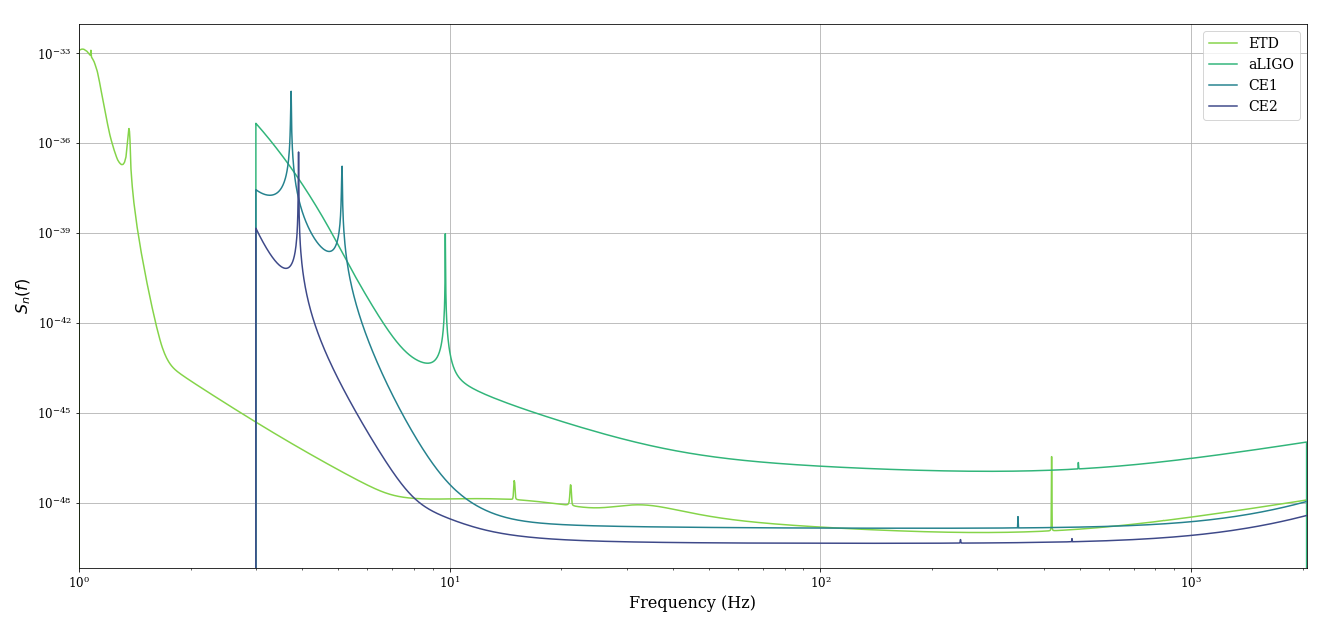
\includegraphics[width=\textwidth]{Figures/Introduction/Noise_curves.png}
    \caption{The detector noise power spectral density (noise curve) for Einstein Telescope (ETD)~\cite{Punturo:2010zz}, Advanced LIGO (aLIGO), and Cosmic Explorer (CE1/CE2)~\cite{Reitze:2019iox} plotted as a function of frequency. The lower frequency limit of Einstein Telescope is $1$~Hz. CE1 and CE2 correspond to the first and second stages of upgrades to Cosmic Explorer. Cosmic Explorer is an order of magnitude more sensitive than Advanced LIGO. The second stage of Cosmic Explorer will further increase the sensitivity.}
    \label{fig:noisecurves}
\end{figure}